\documentclass[11pt,a4paper]{report}
\usepackage[textwidth=37em,vmargin=30mm]{geometry}
\usepackage{calc,xunicode,amsmath,amssymb,paralist,enumitem,tabu,booktabs,datetime2,xeCJK,xeCJKfntef,listings}
\usepackage{tocloft,fancyhdr,tcolorbox,xcolor,graphicx,eso-pic,xltxtra,xelatexemoji}

\newcommand{\envyear}[0]{2025}
\newcommand{\envdatestr}[0]{2025-01-29}
\newcommand{\envfinaldir}[0]{webdb/2025/20250129/final}

\usepackage[hidelinks]{hyperref}
\hypersetup{
    colorlinks=false,
    pdfpagemode=FullScreen,
    pdftitle={Web Digest - \envdatestr}
}

\setlength{\cftbeforechapskip}{10pt}
\renewcommand{\cftchapfont}{\rmfamily\bfseries\large\raggedright}
\setlength{\cftbeforesecskip}{2pt}
\renewcommand{\cftsecfont}{\sffamily\small\raggedright}

\setdefaultleftmargin{2em}{2em}{1em}{1em}{1em}{1em}

\usepackage{xeCJK,xeCJKfntef}
\xeCJKsetup{PunctStyle=plain,RubberPunctSkip=false,CJKglue=\strut\hskip 0pt plus 0.1em minus 0.05em,CJKecglue=\strut\hskip 0.22em plus 0.2em}
\XeTeXlinebreaklocale "zh"
\XeTeXlinebreakskip = 0pt


\setmainfont{Brygada 1918}
\setromanfont{Brygada 1918}
\setsansfont{IBM Plex Sans}
\setmonofont{JetBrains Mono NL}
\setCJKmainfont{Noto Serif CJK SC}
\setCJKromanfont{Noto Serif CJK SC}
\setCJKsansfont{Noto Sans CJK SC}
\setCJKmonofont{Noto Sans CJK SC}

\setlength{\parindent}{0pt}
\setlength{\parskip}{8pt}
\linespread{1.15}

\lstset{
	basicstyle=\ttfamily\footnotesize,
	numbersep=5pt,
	backgroundcolor=\color{black!5},
	showspaces=false,
	showstringspaces=false,
	showtabs=false,
	tabsize=2,
	captionpos=b,
	breaklines=true,
	breakatwhitespace=true,
	breakautoindent=true,
	linewidth=\textwidth
}






\newcommand{\coverpic}[2]{
    % argv: itemurl, authorname
    Cover photo by #2~~(\href{#1}{#1})
}
\newcommand{\makeheader}[0]{
    \begin{titlepage}
        % \newgeometry{hmargin=15mm,tmargin=21mm,bmargin=12mm}
        \begin{center}
            
            \rmfamily\scshape
            \fontspec{BaskervilleF}
            \fontspec{Old Standard}
            \fontsize{59pt}{70pt}\selectfont
            WEB\hfill DIGEST
            
            \vfill
            % \vskip 30pt
            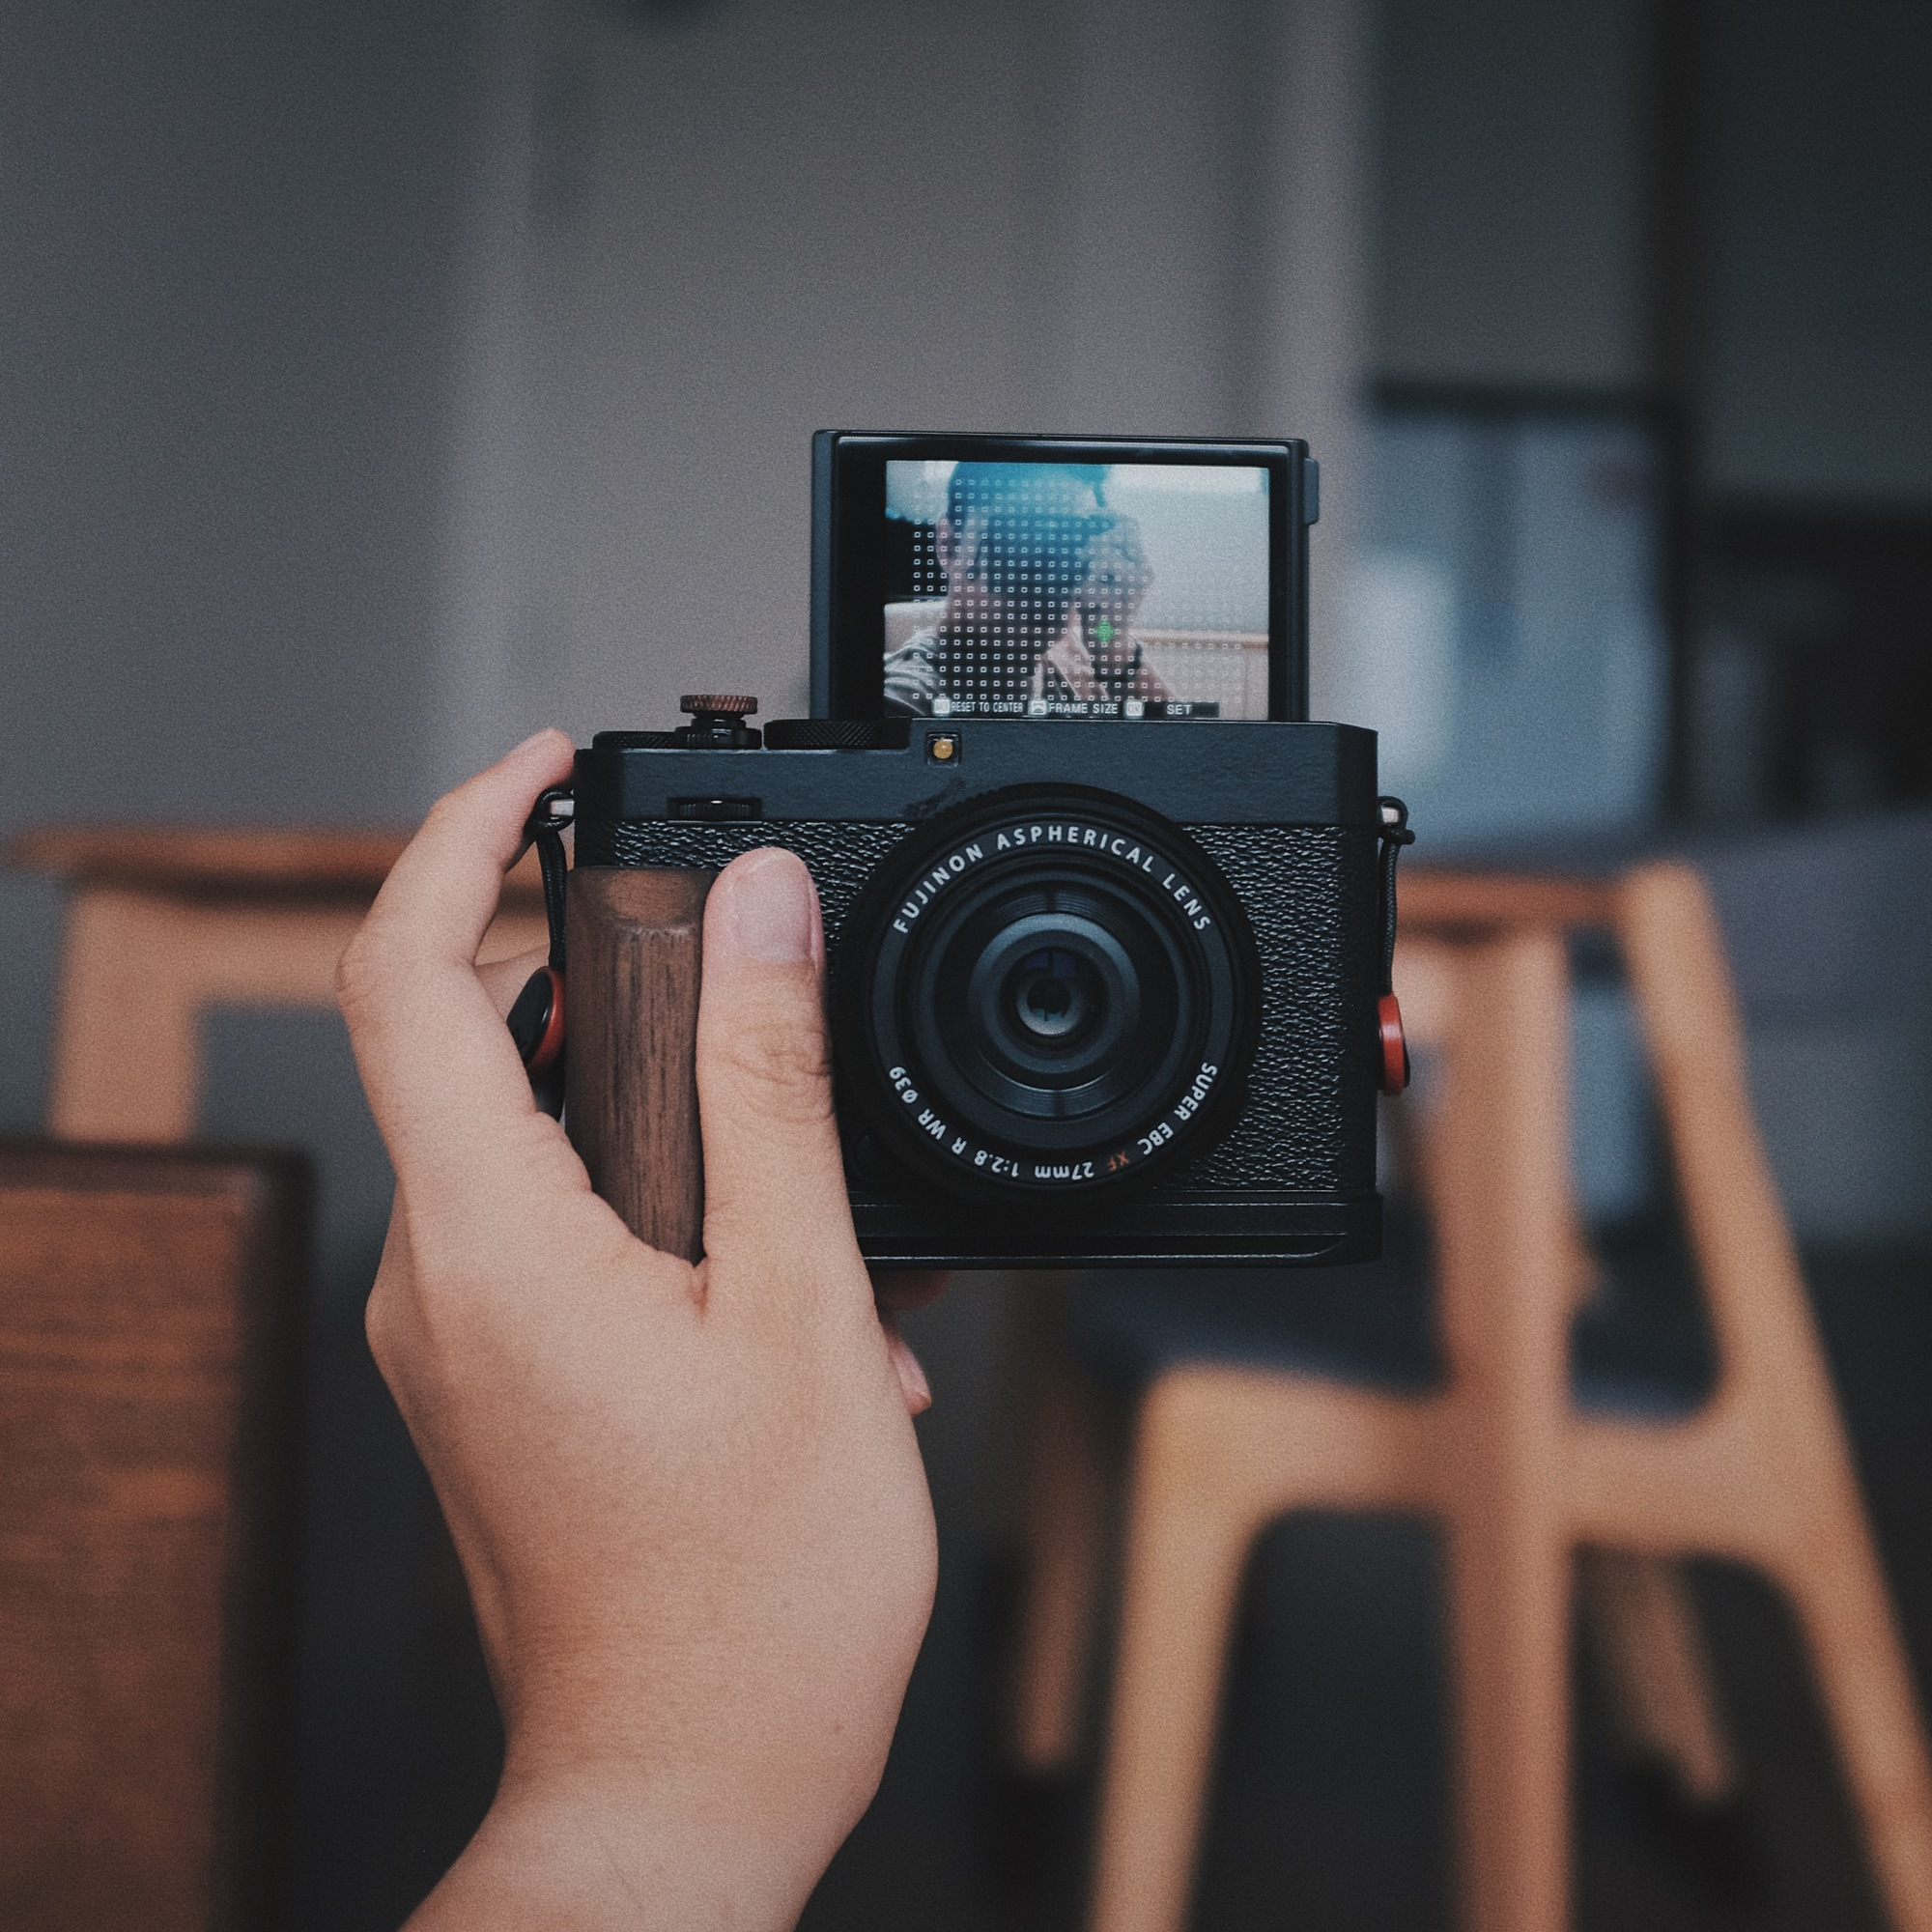
\includegraphics[width=\linewidth]{\envfinaldir/coverpic-prod.jpg}\par
            % \vskip 30pt
            \vfill

            \normalsize\rmfamily\scshape
            \copyright{} The Web Digest Project \hfill\large \envdatestr
        \end{center}
    \end{titlepage}
    % \restoregeometry
}
\newcommand{\simplehref}[1]{%
    \textcolor{blue!80!green}{\href{#1}{#1}}%
}
\renewcommand{\contentsname}{\center\Huge\sffamily\bfseries Contents\par\vskip 20pt}
\newcounter{ipartcounter}
\setcounter{ipartcounter}{0}
\newcommand{\ipart}[1]{
    % \vskip 20pt
    \clearpage
    \stepcounter{ipartcounter}
    \phantomsection
    \addcontentsline{toc}{chapter}{#1}
    % \begin{center}
    %     \Huge
    %     \sffamily\bfseries
    %     #1
    % \end{center}
    % \vskip 20pt plus 7pt
}
\newcounter{ichaptercounter}
\setcounter{ichaptercounter}{0}
\newcommand{\ichapter}[1]{
    % \vskip 20pt
    \clearpage
    \stepcounter{ichaptercounter}
    \phantomsection
    \addcontentsline{toc}{section}{\numberline{\arabic{ichaptercounter}}#1}
    \begin{center}
        \Huge
        \sffamily\bfseries
        #1
    \end{center}
    \vskip 20pt plus 7pt
}
\newcommand{\entrytitlefont}[1]{\subsection*{\raggedright\Large\sffamily\bfseries#1}}
\newcommand{\entryitemGeneric}[2]{
    % argv: title, url
    \parbox{\linewidth}{
        \entrytitlefont{#1}\par\vskip 5pt
        \footnotesize\ttfamily\mdseries
        \simplehref{#2}
    }\vskip 11pt plus 11pt minus 1pt
}
\newcommand{\entryitemGithub}[3]{
    % argv: title, url, desc
    \parbox{\linewidth}{
        \entrytitlefont{#1}\par\vskip 5pt
        \footnotesize\ttfamily\mdseries
        \simplehref{#2}\par\vskip 5pt
        \small\rmfamily\mdseries#3
    }\vskip 11pt plus 11pt minus 1pt
}
\newcommand{\entryitemAp}[3]{
    % argv: title, url, desc
    \parbox{\linewidth}{
        \entrytitlefont{#1}\par\vskip 5pt
        \footnotesize\ttfamily\mdseries
        \simplehref{#2}\par\vskip 5pt
        \small\rmfamily\mdseries#3
    }\vskip 11pt plus 11pt minus 1pt
}
\newcommand{\entryitemHackernews}[3]{
    % argv: title, hnurl, rawurl
    % \parbox{\linewidth}{
    %     \entrytitlefont{#1}\par\vskip 5pt
    %     \footnotesize\ttfamily\mdseries
    %     \simplehref{#3}\par
    %     \textcolor{black!50}{\href{#2}{#2}}
    % }\vskip 11pt plus 11pt minus 1pt
    \begin{minipage}{\linewidth}
            \entrytitlefont{#1}\par\vskip 5pt
            \footnotesize\ttfamily\mdseries
            \simplehref{#3}\par
            \textcolor{black!50}{\href{#2}{#2}}
    \end{minipage}\par\vskip 11pt plus 11pt minus 1pt
}







\begin{document}

\makeheader

\tableofcontents\clearpage




\ipart{Developers}
\ichapter{Hacker News}
\entryitemTwoLinks{DeepSeek's multi-head latent attention and other KV cache tricks}{https://news.ycombinator.com/item?id=42858741}{https://www.pyspur.dev/blog/multi-head-latent-attention-kv-cache-paper-list}

\entryitemTwoLinks{Questions censored by DeepSeek}{https://news.ycombinator.com/item?id=42858552}{https://www.promptfoo.dev/blog/deepseek-censorship/}

\entryitemTwoLinks{Parkinsons patient "feels cured" with new adaptive deep brain stimulation device}{https://news.ycombinator.com/item?id=42857293}{https://www.bbc.com/news/articles/ckgn49r069wo}

\entryitemTwoLinks{New speculative attacks on Apple CPUs}{https://news.ycombinator.com/item?id=42856023}{https://predictors.fail/}

\entryitemTwoLinks{Berkeley Researchers Replicate DeepSeek R1's Core Tech for Just \$30: A Small Mod}{https://news.ycombinator.com/item?id=42855283}{https://xyzlabs.substack.com/p/berkeley-researchers-replicate-deepseek}

\entryitemTwoLinks{Using uv as your shebang line}{https://news.ycombinator.com/item?id=42855258}{https://akrabat.com/using-uv-as-your-shebang-line/}

\entryitemTwoLinks{How has DeepSeek improved the Transformer architecture?}{https://news.ycombinator.com/item?id=42855170}{https://epoch.ai/gradient-updates/how-has-deepseek-improved-the-transformer-architecture}

\entryitemTwoLinks{Sam Altman said startups with \$10M were 'hopeless' competing with OpenAI}{https://news.ycombinator.com/item?id=42854525}{https://www.tomshardware.com/tech-industry/artificial-intelligence/sam-altman-said-startups-with-only-usd10-million-were-totally-hopeless-competing-with-openai-deepseeks-disruption-says-otherwise}

\entryitemTwoLinks{Bitwarden is turning 2FA on by default for new devices}{https://news.ycombinator.com/item?id=42853696}{https://bitwarden.com/help/new-device-verification/}

\entryitemTwoLinks{Boom XB-1 First Supersonic Flight [video]}{https://news.ycombinator.com/item?id=42853633}{https://www.youtube.com/watch?v=-qisIViAHwI}

\entryitemTwoLinks{Almost one in 10 people use the same four-digit PIN}{https://news.ycombinator.com/item?id=42853617}{https://www.abc.net.au/news/2025-01-28/almost-one-in-ten-people-use-the-same-four-digit-pin/103946842}

\entryitemTwoLinks{Maxima in the browser using Embedded Common Lisp on WASM}{https://news.ycombinator.com/item?id=42853528}{https://maxima-on-wasm.pages.dev/}

\entryitemTwoLinks{IAC confirms existence of a Super-earth in the habitable zone of a Sun-like Star}{https://news.ycombinator.com/item?id=42853174}{https://www.iac.es/en/outreach/news/iac-confirms-existence-super-earth-habitable-zone-sun-star}

\entryitemTwoLinks{Promising results from DeepSeek R1 for code}{https://news.ycombinator.com/item?id=42852866}{https://simonwillison.net/2025/Jan/27/llamacpp-pr/}

\entryitemTwoLinks{Janus Pro 1B running 100\% locally in-browser on WebGPU}{https://news.ycombinator.com/item?id=42852400}{https://old.reddit.com/r/LocalLLaMA/comments/1ibnso0/janus\_pro\_1b\_running\_100\_locally\_inbrowser\_on/}

\entryitemTwoLinks{Osaka bans smoking on all of its streets, vaping included}{https://news.ycombinator.com/item?id=42852073}{https://soranews24.com/2025/01/28/osaka-bans-smoking-on-all-of-its-streets-violators-will-be-fined-by-patrols-vaping-included/}

\entryitemTwoLinks{US pauses all federal aid and grants}{https://news.ycombinator.com/item?id=42851248}{https://www.bbc.com/news/articles/c77rdy6gzy5o}

\entryitemTwoLinks{Cleveland police used AI to justify a search warrant. It derailed a murder case}{https://news.ycombinator.com/item?id=42851124}{https://www.cleveland.com/news/2025/01/cleveland-police-used-ai-to-justify-a-search-warrant-it-has-derailed-a-murder-case.html}

\entryitemTwoLinks{US Civil servants are being asked who they voted for in 2024 election}{https://news.ycombinator.com/item?id=42850644}{https://www.independent.co.uk/news/world/americas/us-politics/trump-civil-service-loyalty-transition-b2678674.html}

\entryitemTwoLinks{Run DeepSeek R1 Dynamic 1.58-bit}{https://news.ycombinator.com/item?id=42850222}{https://unsloth.ai/blog/deepseekr1-dynamic}\ichapter{Phoronix}
\entryitemGeneric{\hskip 0pt{}AMD ROCm 6.3.2 Supports Microsoft Azure Linux 3.0, HIP Improvements \& Better Docs}{https://www.phoronix.com/news/AMD-ROCm-6.3.2-Released}

\entryitemGeneric{\hskip 0pt{}Apple CPUs Affected By New SLAP \& FLOP Side-Channel Attacks}{https://www.phoronix.com/news/Apple-CPU-SLAP-FLOP-Attacks}

\entryitemGeneric{\hskip 0pt{}System76's New Linux Mini PC Pairs Intel Meteor Lake + Dual 2.5G Ethernet + Coreboot}{https://www.phoronix.com/news/System76-Meerkat-2025}

\entryitemGeneric{\hskip 0pt{}Raspberry Pi 5 16GB Running Well For Larger Workloads, More Multi-Tasking}{https://www.phoronix.com/review/raspberry-pi-5-16gb}

\entryitemGeneric{\hskip 0pt{}Thunderbolt 3 AltMode Driver \& Other USB Improvements For Linux 6.14}{https://www.phoronix.com/news/Linux-6.14-USB-Thunderbolt}

\entryitemGeneric{\hskip 0pt{}WavPack 5.8 Lossless Audio Compression Tools Now Enable Multi-Threading By Default}{https://www.phoronix.com/news/WavPack-5.8-Released}

\entryitemGeneric{\hskip 0pt{}LLVM 20 Promotes SPIR-V To Official Backend, Enabled By Default}{https://www.phoronix.com/news/LLVM-20-SPIR-V-Official-Target}

\entryitemGeneric{\hskip 0pt{}F2FS Improvements Merged For Linux 6.14}{https://www.phoronix.com/news/Linux-6.14-F2FS}

\entryitemGeneric{\hskip 0pt{}Z3fold Allocator Slated For Removal From The Linux Kernel}{https://www.phoronix.com/news/Linux-Z3fold-Removal-Coming}\ichapter{Dribbble}
\entryitemGeneric{\hskip 0pt{}DeepSeek logo redesign}{https://dribbble.com/shots/25543483-DeepSeek-logo-redesign}

\entryitemGeneric{\hskip 0pt{}Apparel}{https://dribbble.com/shots/25538973-Apparel}

\entryitemGeneric{\hskip 0pt{}B}{https://dribbble.com/shots/25536900-B}

\entryitemGeneric{\hskip 0pt{}De Nieuwe Gemeente - Church Brand}{https://dribbble.com/shots/25537128-De-Nieuwe-Gemeente-Church-Brand}

\entryitemGeneric{\hskip 0pt{}Speed Test App Ui Design}{https://dribbble.com/shots/25535763-Speed-Test-App-Ui-Design}

\entryitemGeneric{\hskip 0pt{}2024 Logo Design Recap Pt.1}{https://dribbble.com/shots/25534698-2024-Logo-Design-Recap-Pt-1}

\entryitemGeneric{\hskip 0pt{}Plexo mobile app}{https://dribbble.com/shots/25534405-Plexo-mobile-app}

\entryitemGeneric{\hskip 0pt{}Dyna - Logo Design}{https://dribbble.com/shots/25525428-Dyna-Logo-Design}

\entryitemGeneric{\hskip 0pt{}Godzilla Logo}{https://dribbble.com/shots/25525727-Godzilla-Logo}

\entryitemGeneric{\hskip 0pt{}B}{https://dribbble.com/shots/25524895-B}

\entryitemGeneric{\hskip 0pt{}Peregrine Engineering®}{https://dribbble.com/shots/25527465-Peregrine-Engineering}

\entryitemGeneric{\hskip 0pt{}VCC Unused Logo Concept - V4}{https://dribbble.com/shots/25525024-VCC-Unused-Logo-Concept-V4}

\entryitemGeneric{\hskip 0pt{}2024 Logo Design Recap Pt.1}{https://dribbble.com/shots/25525396-2024-Logo-Design-Recap-Pt-1}

\entryitemGeneric{\hskip 0pt{}M for Mountain Logo Design (Unused for Sale)}{https://dribbble.com/shots/25524897-M-for-Mountain-Logo-Design-Unused-for-Sale}

\entryitemGeneric{\hskip 0pt{}Tattooed Devil Horns}{https://dribbble.com/shots/25520911-Tattooed-Devil-Horns}

\entryitemGeneric{\hskip 0pt{}Fitness and Step Count app UI Design}{https://dribbble.com/shots/25518949-Fitness-and-Step-Count-app-UI-Design}

\entryitemGeneric{\hskip 0pt{}Carbon Solutions B2B Dashboard Design}{https://dribbble.com/shots/25506638-Carbon-Solutions-B2B-Dashboard-Design}

\entryitemGeneric{\hskip 0pt{}Goose Gym}{https://dribbble.com/shots/25515121-Goose-Gym}

\entryitemGeneric{\hskip 0pt{}Product design - icons set}{https://dribbble.com/shots/25516253-Product-design-icons-set}

\entryitemGeneric{\hskip 0pt{}Rapid Rabbit Logo}{https://dribbble.com/shots/25516738-Rapid-Rabbit-Logo}

\entryitemGeneric{\hskip 0pt{}LLM GPU Manager}{https://dribbble.com/shots/25513811-LLM-GPU-Manager}

\entryitemGeneric{\hskip 0pt{}HappyDev - Logo Design / Branding}{https://dribbble.com/shots/25514894-HappyDev-Logo-Design-Branding}

\entryitemGeneric{\hskip 0pt{}VCC Unused Logo Design Concept}{https://dribbble.com/shots/25511334-VCC-Unused-Logo-Design-Concept}

\entryitemGeneric{\hskip 0pt{}The Toucan}{https://dribbble.com/shots/25515890-The-Toucan}


\ipart{Developers~~~~(zh-Hans)}
\ichapter{Solidot}
\entryitemGeneric{\hskip 0pt{}研究估计到 2100 年欧洲高温死亡人数增加五成}{https://www.solidot.org/story?sid=80443}

\entryitemGeneric{\hskip 0pt{}Google 开源 Pebble 智能手表操作系统}{https://www.solidot.org/story?sid=80442}

\entryitemGeneric{\hskip 0pt{}用开源方法复现 DeepSeek-R1}{https://www.solidot.org/story?sid=80441}

\entryitemGeneric{\hskip 0pt{}Onlyfans 成功背后的心理学}{https://www.solidot.org/story?sid=80440}

\entryitemGeneric{\hskip 0pt{}科学家通过黑洞合并事件验证宇宙镜像对称性}{https://www.solidot.org/story?sid=80439}

\entryitemGeneric{\hskip 0pt{}研究揭示 PM2.5 毒理学机制}{https://www.solidot.org/story?sid=80438}

\entryitemGeneric{\hskip 0pt{}DeepSeek 登顶苹果应用商店免费应用排行榜}{https://www.solidot.org/story?sid=80437}

\entryitemGeneric{\hskip 0pt{}天文学家呼吁禁止太空广告}{https://www.solidot.org/story?sid=80436}

\entryitemGeneric{\hskip 0pt{}研究发现对 AI 了解越少的人越愿意使用 AI}{https://www.solidot.org/story?sid=80435}

\entryitemGeneric{\hskip 0pt{}特斯拉拒绝将 FSD 软件转移到新车}{https://www.solidot.org/story?sid=80434}

\entryitemGeneric{\hskip 0pt{}Bitmanagement 与美国海军的反盗版诉讼再次受挫}{https://www.solidot.org/story?sid=80433}

\entryitemGeneric{\hskip 0pt{}GLP-1RA 的益处和风险}{https://www.solidot.org/story?sid=80431}

\entryitemGeneric{\hskip 0pt{}研究人员发现中欧电网用非加密无线信号控制}{https://www.solidot.org/story?sid=80430}

\entryitemGeneric{\hskip 0pt{}甲骨文等正在谈判接手 TikTok 美国业务}{https://www.solidot.org/story?sid=80428}

\entryitemGeneric{\hskip 0pt{}小鼠研究发现微塑料会堵塞大脑血液流动}{https://www.solidot.org/story?sid=80427}

\entryitemGeneric{\hskip 0pt{}ADHD 患者有更短的预期寿命}{https://www.solidot.org/story?sid=80426}

\entryitemGeneric{\hskip 0pt{}研究称电动汽车的寿命与燃油汽车相差无几}{https://www.solidot.org/story?sid=80425}

\entryitemGeneric{\hskip 0pt{}大英博物馆遭前 IT 雇员攻击而部分关闭}{https://www.solidot.org/story?sid=80424}\ichapter{V2EX}
\entryitemGeneric{\hskip 0pt{}[macOS] 买大内存 MacBook 的一个意外好处——私人 AI 服务器}{https://www.v2ex.com/t/1108245}

\entryitemGeneric{\hskip 0pt{}[宁波] NB 的 V 油们!}{https://www.v2ex.com/t/1108244}

\entryitemGeneric{\hskip 0pt{}[VPS] 美国洛杉矶 vps 万兆 4837|9929+CMIN2|CN2GIA 月付全场 8.5 永久折扣!}{https://www.v2ex.com/t/1108243}

\entryitemGeneric{\hskip 0pt{}[OpenAI] Janus Pro: A Revolutionary AI Model}{https://www.v2ex.com/t/1108242}

\entryitemGeneric{\hskip 0pt{}[问与答] Apple Intelligent 是不是可以直接找 deepseek 谈合作了}{https://www.v2ex.com/t/1108241}

\entryitemGeneric{\hskip 0pt{}[问与答] 电脑经常死机,求各位大佬帮忙分析下是哪个部件出问题了}{https://www.v2ex.com/t/1108240}

\entryitemGeneric{\hskip 0pt{}[奇思妙想] 从语言编码到发展原因的一种可能性}{https://www.v2ex.com/t/1108239}

\entryitemGeneric{\hskip 0pt{}[OpenWrt] lan ipv4 的设备可以通过 wan ipv6 进行端口映射吗?}{https://www.v2ex.com/t/1108238}

\entryitemGeneric{\hskip 0pt{}[分享发现] 家里老人被骗十万买了所谓的频谱治疗屋,农村保健品销售乱象}{https://www.v2ex.com/t/1108237}

\entryitemGeneric{\hskip 0pt{}[4G] 漫游卡漫游到中国(内地)只能用 4G 且不能使用 VoLTE 吗?}{https://www.v2ex.com/t/1108235}

\entryitemGeneric{\hskip 0pt{}[分享创造] 趁着春节更新了一下自己开源的 DualSense 测试网站,支持了 DualSenseEdge}{https://www.v2ex.com/t/1108234}

\entryitemGeneric{\hskip 0pt{}[生活] 在这个除夕夜,我的 iPhone15Pro 完成了``自我划痕''}{https://www.v2ex.com/t/1108233}

\entryitemGeneric{\hskip 0pt{}[Apple] 用户称 MacBook Pro 车祸中被毁, AppleCare+ 拒赔}{https://www.v2ex.com/t/1108232}

\entryitemGeneric{\hskip 0pt{}[生活] 大过年的停电了...}{https://www.v2ex.com/t/1108231}

\entryitemGeneric{\hskip 0pt{}[生活] 春晚只为看王菲}{https://www.v2ex.com/t/1108230}

\entryitemGeneric{\hskip 0pt{}[问与答] 今年春晚演的啥}{https://www.v2ex.com/t/1108229}

\entryitemGeneric{\hskip 0pt{}[问与答] iPhone 没电没法开机,充电貌似都充不进去}{https://www.v2ex.com/t/1108227}

\entryitemGeneric{\hskip 0pt{}[Apple] 库克等级森严使我 air 无力战胜 HDR 剪辑}{https://www.v2ex.com/t/1108226}

\entryitemGeneric{\hskip 0pt{}[随想] 很不喜欢岳云鹏的相声}{https://www.v2ex.com/t/1108225}

\entryitemGeneric{\hskip 0pt{}[Linux] 请问安装好了极光面板,但后台显示部署失败,为什么出现 STDOUT No stdout found!}{https://www.v2ex.com/t/1108223}

\entryitemGeneric{\hskip 0pt{}[生活] 新年快樂! Happy Chinese New Year!}{https://www.v2ex.com/t/1108222}

\entryitemGeneric{\hskip 0pt{}[问与答] 有没有和我一样觉得走亲戚式拜年太耗精力?}{https://www.v2ex.com/t/1108221}

\entryitemGeneric{\hskip 0pt{}[生活] 2025-01-28.与父亲的一次面谈}{https://www.v2ex.com/t/1108220}

\entryitemGeneric{\hskip 0pt{}[程序员] 电子专业跨行学算法有推荐路径吗}{https://www.v2ex.com/t/1108219}

\entryitemGeneric{\hskip 0pt{}[生活] 商业保险:购买原研药的最佳选择?}{https://www.v2ex.com/t/1108218}

\entryitemGeneric{\hskip 0pt{}[问与答] ansible 或 terraform 有没有方法获得刚创建的 ec2 实例的 public ip?}{https://www.v2ex.com/t/1108217}

\entryitemGeneric{\hskip 0pt{}[问与答] 有使用 vscode 的 Copilot Edit 的吗?}{https://www.v2ex.com/t/1108216}

\entryitemGeneric{\hskip 0pt{}[分享创造] 开发了一个 AI 生成图片网站}{https://www.v2ex.com/t/1108215}

\entryitemGeneric{\hskip 0pt{}[分享创造] [附兑换码] Moeli 阅读,简单易用的电子书阅读器}{https://www.v2ex.com/t/1108214}

\entryitemGeneric{\hskip 0pt{}[生活] 过年回家,现在感觉很窒息}{https://www.v2ex.com/t/1108213}

\entryitemGeneric{\hskip 0pt{}[JetBrains] webstorm 新版本在全局搜索中取消了模块选项卡}{https://www.v2ex.com/t/1108212}

\entryitemGeneric{\hskip 0pt{}[YouTube] YouTube 重度用户,回答一些分区经常看见的问题}{https://www.v2ex.com/t/1108210}

\entryitemGeneric{\hskip 0pt{}[游戏] 闲蛋疼,启动王者荣耀}{https://www.v2ex.com/t/1108209}

\entryitemGeneric{\hskip 0pt{}[分享发现] 各位年夜饭都是什么啊}{https://www.v2ex.com/t/1108208}

\entryitemGeneric{\hskip 0pt{}[分享创造] 交互式音乐教程增加新功能 [调音器] https://lightnote.com.cn/tuner}{https://www.v2ex.com/t/1108207}

\entryitemGeneric{\hskip 0pt{}[iOS] ios 一个严重 bug}{https://www.v2ex.com/t/1108205}

\entryitemGeneric{\hskip 0pt{}[Apple] iOS 18.3 仍然没有修复后台任务卡片色彩过饱和的问题}{https://www.v2ex.com/t/1108204}

\entryitemGeneric{\hskip 0pt{}[汽车] 车辆被撞}{https://www.v2ex.com/t/1108203}

\entryitemGeneric{\hskip 0pt{}[分享发现] 一款免费、开源的在线背景图生成器,请各位帮我在 ProductHunt 上面投一票!}{https://www.v2ex.com/t/1108202}

\entryitemGeneric{\hskip 0pt{}[问与答] 我现在为什么讨厌 Bitget(重发)}{https://www.v2ex.com/t/1108199}

\entryitemGeneric{\hskip 0pt{}[iOS] 给老年人用的 iOS 第三方美颜相机,求推荐}{https://www.v2ex.com/t/1108198}

\entryitemGeneric{\hskip 0pt{}[问与答] 如果苹果国内使用的是 deepseek,你们还会买国行吗?}{https://www.v2ex.com/t/1108196}

\entryitemGeneric{\hskip 0pt{}[Apple] ip16 pm 美版在国内怎么没有卫星通讯应用?}{https://www.v2ex.com/t/1108194}

\entryitemGeneric{\hskip 0pt{}[OpenAI] 兄弟们 o1 和 o1 mini 炸了 model not found}{https://www.v2ex.com/t/1108192}

\entryitemGeneric{\hskip 0pt{}[生活] 好多 AI 都识别不出来这是啥字}{https://www.v2ex.com/t/1108191}

\entryitemGeneric{\hskip 0pt{}[信息安全] 如果 AES 无法用 GCM 模式,用明文 hash 作为 IV 以实现完整性校验是一个好的实现吗?}{https://www.v2ex.com/t/1108190}

\entryitemGeneric{\hskip 0pt{}[程序员] 有支持加密存储的 NVR 硬盘录像机吗}{https://www.v2ex.com/t/1108189}

\entryitemGeneric{\hskip 0pt{}[问与答] 小白请教下 deepseek 本地部署有什么优势吗?以及个人一点设想}{https://www.v2ex.com/t/1108188}

\entryitemGeneric{\hskip 0pt{}[酷工作] 有啥远程兼职可以做做的嘛}{https://www.v2ex.com/t/1108187}


\ipart{Generic News}
\ichapter{AP News}
\entryitemWithDescription{\hskip 0pt{}Caroline Kennedy warns senators that cousin RFK Jr. is a `predator'}{https://apnews.com/article/f01f58305eac53560e31c51aaee5f171}{}

\entryitemWithDescription{\hskip 0pt{}Watch a miles-long cluster of dolphins captured on drone video}{https://apnews.com/article/6fd383a160f4a49340cccc8d8a983d3b}{}

\entryitemWithDescription{\hskip 0pt{}Jake, Logan Paul make cryptic HBO Max announcements on social media}{https://apnews.com/article/8bb77544572adeb2f1879a9e17f9f2b3}{}

\entryitemWithDescription{\hskip 0pt{}A\$AP Rocky's accuser is testifying at his shooting trial in LA}{https://apnews.com/article/8624e88e781aa738a6ae1b2525f6e641}{}

\entryitemWithDescription{\hskip 0pt{}Voting rights groups are concerned about priorities shifting under Trump's Justice Department}{https://apnews.com/article/28ffe85f81e7edf95064e5192c3efce1}{}

\entryitemWithDescription{\hskip 0pt{}How the Los Angeles wildfires will transform the 2025 Grammys}{https://apnews.com/article/99be63665abdf38bfb50315fdab6b339}{}

\entryitemWithDescription{\hskip 0pt{}Blake Lively and Justin Baldoni get March 2026 trial date for her `It Ends With Us' lawsuit}{https://apnews.com/article/9f40635a679b8e505fd403a337e1ad85}{}

\entryitemWithDescription{\hskip 0pt{}Chinese tech startup DeepSeek says it was hit with `large-scale malicious attacks'}{https://apnews.com/article/be414acadbf35070d7645fe9fbd8f464}{}

\entryitemWithDescription{\hskip 0pt{}Full-scale replica of Anne Frank's hidden annex opens in NYC}{https://apnews.com/article/b2490ae41d4fe9fcb895fb4ed12147ab}{}

\entryitemWithDescription{\hskip 0pt{}Chiefs look to join the Shaq-Kobe Lakers, Yankees and Michael Jordan with a rare three-peat}{https://apnews.com/article/de191c6b32e9835f479a965ef2f8373d}{}

\entryitemWithDescription{\hskip 0pt{}Spectator is killed by a stray hammer thrown at a Colorado youth track and field meet}{https://apnews.com/article/530ea88da9c43fe4ec9aed1f2a1b8b4f}{}

\entryitemWithDescription{\hskip 0pt{}The Chiefs get more Mahomes magic and advance to 3rd straight Super Bowl, beating the Bills 32-29}{https://apnews.com/article/c9187ccf15160bd5eabba73086ee9a42}{}

\entryitemWithDescription{\hskip 0pt{}Percival Everett's `James' awarded Carnegie Medal for fiction}{https://apnews.com/article/699ca2d278b43dd7bd515792b5d7fe3a}{}






\clearpage
\leavevmode\vfill
\footnotesize

Copyright \copyright{} 2023-2025 Neruthes and other contributors.

This document is published with CC BY-NC-ND 4.0 license.

The entries listed in this newsletter may be copyrighted by their respective creators.

This newsletter is generated by the Web Digest project.

The newsletters are also delivered via Telegram channel \CJKunderline{\href{https://t.me/webdigestchannel}{https://t.me/webdigestchannel}}.\\
RSS feed is available at \CJKunderline{\href{https://webdigest.pages.dev/rss.xml}{https://webdigest.pages.dev/rss.xml}}.

This newsletter is available in PDF at
\CJKunderline{\href{https://webdigest.pages.dev/}{https://webdigest.pages.dev/}}.

The source code being used to generate this newsletter is available at\\
\CJKunderline{\href{https://github.com/neruthes/webdigest}{https://github.com/neruthes/webdigest}}.

This newsletter is also available in
\CJKunderline{\href{http://webdigest.pages.dev/readhtml/\envyear/WebDigest-20250129.html}{HTML}} and
\CJKunderline{\href{https://github.com/neruthes/webdigest/blob/master/markdown/\envyear/WebDigest-20250129.md}{Markdown}}.


\coverpic{https://unsplash.com/photos/a-church-filled-with-lots-of-pews-next-to-tall-windows-UVL\_Ix960es}{Luca Cavallin}


\end{document}
